\documentclass[t]{beamer}
\setlength{\parindent}{0em}
\setlength{\parskip}{2cm}
% Max: 121.92 x 121.92
\usepackage[orientation=landscape,size=custom,width=110,height=90,scale=1]{beamerposter}
%\usepackage{lmodern} % Font style

\usepackage{natbib}

\usepackage{enumitem}
\setlist[description]{style=nextline, itemsep=1cm}

\usefonttheme{serif}
\usepackage{ragged2e} % For using \justify
\usepackage{url}
\usepackage{graphicx}
\graphicspath{{Figures/}}

% texpos package divides poster into columns and sections (relative or absolute positions)
%\usepackage[absolute,overlay]{textpos} ??
\usepackage[absolute, overlay]{textpos}


% Colors, fonts, et.
\definecolor{arsenic}{rgb}{0.23, 0.27, 0.29}

% Whole frame
\setbeamercolor{background canvas}{bg=white}
\setbeamercolor{frametitle}{fg=arsenic}
\setbeamercolor{framesubtitle}{fg=arsenic}

\addtobeamertemplate{frametitle}{\vspace*{5cm}}{\vspace*{-5cm}}
\setbeamertemplate{frametitle}[default][center]
\setbeamerfont{frametitle}{size=\Huge, series=\bfseries}
\setbeamerfont{framesubtitle}{size=\LARGE}

% Blocks
%\setbeamerfont{block title}{size=\LARGE}
\setbeamerfont{block body}{size=\large}
\setbeamercolor{block title}{fg=white, bg=arsenic}
\setbeamercolor{block body}{bg=white, fg=black}
\addtobeamertemplate{block begin}{\vspace*{40pt}}{}
\newcommand{\myblock}[1]{\LARGE\thesection. #1 \vspace{1cm}}

% Normal text
\setbeamercolor{normal text}{fg=black}
%\setbeamerfont{normal text}{size=\fontsize{24pt}{26pt}\selectfont}


% Captions
\usepackage{caption}
\setbeamertemplate{caption}[numbered]
\setbeamerfont{caption}{size=\small}
\setbeamercolor{caption name}{fg=arsenic}

\setbeamertemplate{itemize items}{$\circ$}
\setbeamercolor{description item}{fg=black}
\setbeamercolor{enumerate item}{fg=black}

\setbeamersize{text margin left=3cm,text margin right=3cm}

% Different colors for lightcurve plot, increase font size too
% Print copies of poster?
% Print abstract?
% Linkedin, my info, resume, etc.
% Add twitter, facebook, github, whatev. to poster itself

\usepackage[listings,theorems]{tcolorbox}


\begin{document}

\begin{frame}[t]
    \frametitle{ \vspace{1cm}

    Determining coronal bright point size using
    cross-correlation techniques and data from AIA/\textit{SDO}}
    \framesubtitle{Laurel Farris$^{1}$, R. T. James McAteer$^{1}$}
    \begin{center}
        \textcolor{arsenic}{$^{1}$New Mexico State University}
    \end{center}

    \setbeamercolor{normal text}{fg=black}
    \tcbset{
        colback=white, %blue!5,
        colframe=arsenic, %blue!75!black,
        fonttitle={\LARGE\bfseries\thesection. } ,
        enlarge bottom by=10mm,
        boxsep=8mm, % space between box edges and text
        arc=10mm,
        }
    \begin{columns}[t]
        \column{0.3\textwidth}
        \section{}

        \begin{tcolorbox}[title=Introduction]
            \begin{description}
                \item [Background]
                    Coronal bright points (CBPs) are seen ubiquitously in the solar atmosphere
                    at several EUV and X-ray bandpasses. They are thought to be
                    associated with converging areas of magnetic flux at
                    opposite polarities.
                \begin{figure}[t]
                    \vspace{1cm}
                    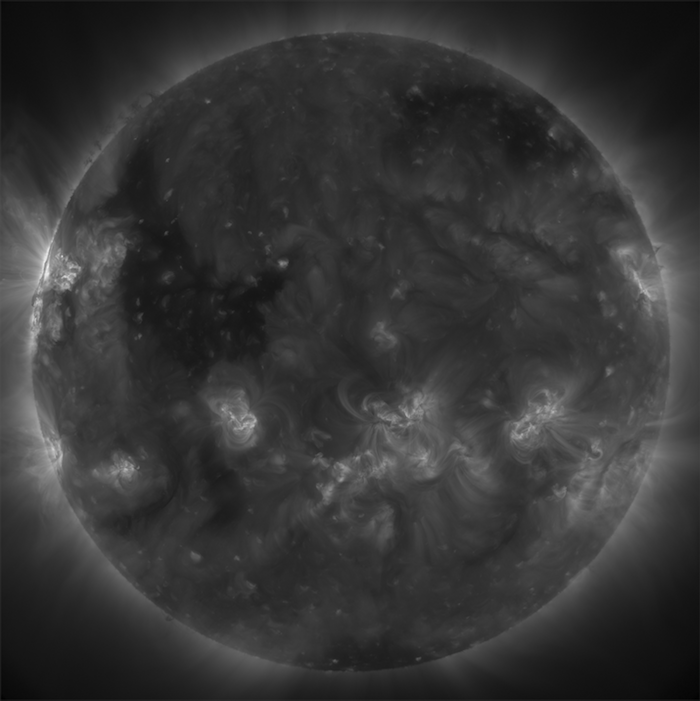
\includegraphics[width=0.8\textwidth]{full_disk.png}\\
                    \parbox{0.8\textwidth}{\caption{Full disk in AIA 193\AA{} bandpass.
                        A coronal hole is present in the upper left region.}}
                \end{figure}
                \item [Motivation]
                    Previously, the size of CBPs has been
                    determined using the intensity at a single point in time,
                    compared to the background intensity.
            \end{description}
        \end{tcolorbox}

        \section{}
        \begin{tcolorbox}[title=Observations]
            \begin{columns}
                \column{0.5\textwidth}
                \column{0.5\textwidth}
                The Atmospheric Imaging Assembly (AIA)
                on board the \textit{Solar Dynamics Observatory (SDO)} obtains
                images at a cadence of 12 seconds over multiple EUV bandpasses.
                Six of these were investigated here to compare the results
                over different
                temperatures/heights in the solar corona.
            \end{columns}
        \end{tcolorbox}

        \column{0.3\textwidth}
        \section{}
        \begin{tcolorbox}[title=Methods]
            \begin{description}[style=nextline]
                \item [Mathematical] The formula for cross-correlation is
                    given by:
                    \[
                        f(t) \star g(t) \equiv f(t) \ast g(-t)
                        \]
                \item [Numerical] For programming, the cross-correlation
                    is calculated using:
                    \[
                        \sum_{0}^{N-1}
                        \]
            \end{description}
        \end{tcolorbox}

        \column{0.3\textwidth}

        \section{}
        \begin{tcolorbox}[title=Results]
            By employing the algorithm from McIntosh et al. (2008),
            the inner structure of the CBP was revealed, most apparent
            in the 193\AA{} data. By cross-correlating each reference
            pixel with every other pixel in the image, a ring-shaped
            structure was revealed around this core, with low values
            of cross-correlation in between.

        \end{tcolorbox}

        \section{}
        \begin{tcolorbox}[title=Conclusion]

        \end{tcolorbox}

    \tcbset{
        fonttitle={\large\bfseries} ,
        }
        \begin{tcolorbox}[title=References]
%           \begin{thebibliography}
%               \bibitem[McIntosh et al. (2008)]{McIntosh}
%                @ARTICLE{McIntosh,
%                   author = {{McIntosh}, S.~W. and {de Pontieu}, B. and {Tomczyk}, S.},
%                    title = "{A Coherence-Based Approach for Tracking Waves in the Solar Corona}",
%                  journal = {\solphys},
%                archivePrefix = "arXiv",
%                   eprint = {0808.2978},
%                 keywords = {Coronal seismology, Oscillations, Solar, Waves, Waves, Magnetohydrodynamic},
%                     year = 2008,
%                    month = nov,
%                   volume = 252,
%                    pages = {321-348},
%                      doi = {10.1007/s11207-008-9257-x},
%                   adsurl = {http://adsabs.harvard.edu/abs/2008SoPh..252..321M},
%                  adsnote = {Provided by the SAO/NASA Astrophysics Data System}
%                }
%           \end{thebibliography}
        \end{tcolorbox}

    \end{columns}

\vfill


\includegraphics[width=0.08\textwidth]{nmsu-logo.jpg}
\end{frame}
\end{document}
